\chapter{Results}

\label{chap:results}

The experiments were conducted using the PostgreSQL 9.0.7 as the database system. Because of the nature of the advisor, all tests were performed on a single host from a cluster managed by OpenNebula 3.6. The host has one 2.4GHz dual core processor and 4GB RAM, running Fedora Linux 16, using kernel version 3.3.8. Even though the the library created to reallocate CPU in OpenRC should work with all the hypervisors supported by Libvirt, the experiments were only performed with KVM\footnote{http://www.linux-kvm.org/}. This hypervisor is already integrated within the mainline Linux kernel since the 2.6.0 kernel version. It only supports hardware virtualization.

During the calibration step, a special VM was created to be run on newly added hosts. It runs the Debian Squeeze Linux operating system, specially configured to be a database server. It contains a 300MB TPC-B database, created with PGBench. Under the tested host, the VM was given both CPUs and 2GB of RAM. Considering the database size, the whole database is loaded in memory. This decision does not have any impact, since only the parameters that describe CPU should be calibrated, instead of I/O. The memory storage for PostgreSQL was created using standard features provided by the DBMS and Linux operating system. The PostgreSQL init scripts were modified to automatically handle this storage every time the database service is stopped or started, including the VM booting. As the calibration queries have a simple known query plan, all the tuning parameters are only modified if their change has an effect in the query optimizer decisions. Otherwise, their default values are not modified.

The parameters \textbf{cpu\_tuple\_cost} and \textbf{cpu\_operator\_cost} were calibrated using the query shown in  ~\ref{app:cal1}. The values obtained for different resource allocations are shown in figures ~\ref{fig:cpuop} and ~\ref{fig:cputp}, along with the linear regression performed on them. Based on these results, it is possible to observe that the parameters that describe CPU do not have a strict linear variation, as seen on  \cite{4401021}. However it contradicts  \cite{Soror:2008:AVM:1376616.1376711}, which affirmed that this variation was linear when the memory for the VM was allocated to $50\%$. Considering the linear equation to be
\[
 f(x) = m*x + b
\],
the asymptotic errors found were the following:
\begin{itemize}
 \item \textbf{cpu\_tuple\_cost}
 \begin{itemize}
  \item $m \approx 6,7\% $;
  \item $b \approx 3,9\% $;
 \end{itemize}
  \item \textbf{cpu\_operator\_cost}
 \begin{itemize}
  \item $m \approx 9.2\% $;
  \item $b \approx 5.6\% $.
 \end{itemize}
\end{itemize}

 
 \begin{figure}[ht]
 \centering
 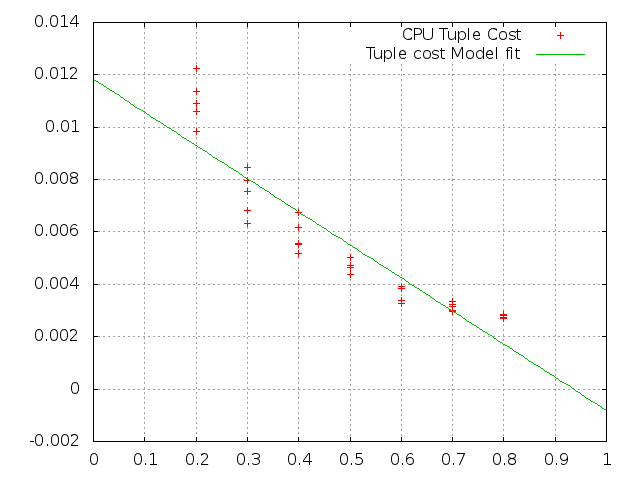
\includegraphics[width=0.8\textwidth]{cpu-operator-cost.png}
 \caption{$cpu\_operator\_cost$ calibration}
 \label{fig:cpuop}
 \end{figure} 
% 
% 
 \begin{figure}[ht]
 \centering
 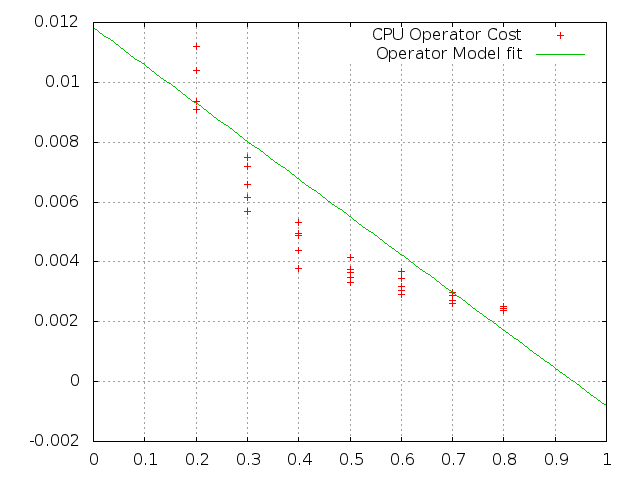
\includegraphics[width=0.8\textwidth]{cpu-tuple-cost.png}
 \caption{$cpu\_tuple\_cost$ calibration}
 \label{fig:cputp}
 \end{figure} 
 
 The calibration of the parameter \textbf{cpu\_index\_tuple} was performed according to chapter \label{chap:implementation}. The results were obtained through the execution of the query presented in subsection \label{app:cal2}. They are shown in figure ~\ref{fig:cpuip}. The errors found for linear parameters $m$ and $b$ are approximately $8.6\%$ and $5.1\%$ , respectively.

 \begin{figure}[ht]
 \centering
 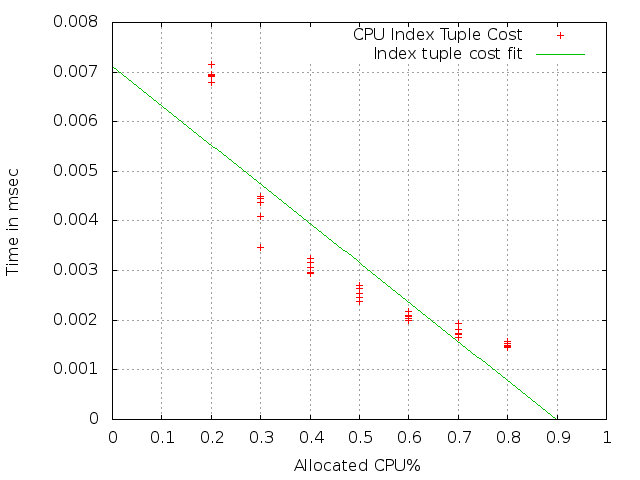
\includegraphics[width=0.8\textwidth]{cpu-index-tuple-cost.png}
 \caption{$cpu\_index\_tuple\_cost$ calibration}
 \label{fig:cpuip}
 \end{figure} 
 
 Once the descriptive parameters are calibrated, it is possible to test the advisor. The tests were performed using TPC-H databases with scale factor 0.6. With indexes, the size of these databases is $4339 MB$. In order to minimize I/O effects, the databases are also loaded  in a RAM based file system, even though they will not fit entirely in the available RAM. Each database runs in a VM with $1.8 GB$ of RAM.
 
 To measure the performance of our advisor, we compare the costs of running the workloads under the recommended resource allocation to the default allocation. The default is to simply allocate $1/N$ of the available CPU to the $N$ virtual machines. We consider $T_{default}$ and $T_{advisor}$ to be the execution time of the $N$ workloads running under the default resource allocation and the recommended one, respectively. The performance metric, defined in \cite{Soror:2008:AVM:1376616.1376711}, is the following:
 \[
  \frac{T_{default}-T_{advisor}}{T_{default}}
 \]
.
